
\chapter{RESULTADOS}

A seguir são apresentados os resultados obtidos ...

\section{Secao 1}
\label{sec:Secao_1}
Na figura \ref{fig:figura50}...

\begin{figure}[H]
    \centering
    \caption{Testes 1}
    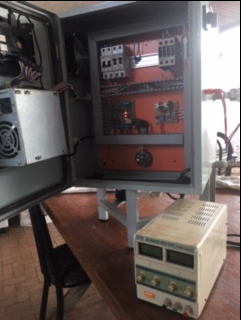
\includegraphics[width=0.6\textwidth]{figuras/figu50.png}
    \fonte{Alguem lugar sujo}
    \label{fig:figura50}
\end{figure}

\section{Secao 2}
\label{sec:Secao_2}

Na figura \ref{fig:figura44}, foi realizado ....

\begin{figure}[H]
    \centering
    \caption{Testes 2}
    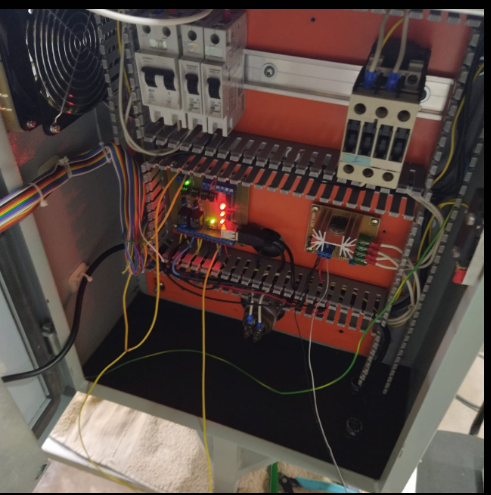
\includegraphics[width=0.6\textwidth]{figuras/figu44.png}
    \fonte{O mesmo lugar sujo}
    \label{fig:figura44}
\end{figure}

Não foi possível realizar e finalizar todos os testes como: ... devido a pandemia do $COVI19$ de acordo com o DECRETO No 64.864, no dia 16 de março de 2020,onde as atividades em sala de aula, que eram presenciais, ficaram suspensas, e também teve início o distanciamento social